\documentclass{article}
\usepackage{amsmath}
\usepackage[UTF8, fontset=none]{ctex} % 禁用默认字体
\usepackage{fontspec}
\usepackage{graphicx}
\setmainfont{Noto Sans CJK SC}
\title{射电干涉测量原理与基线转换公式}

\begin{document}
\maketitle
\section{干涉测量核心方程}
复可见度表示为:
\begin{equation}
V(u,v,w) = \iint I(l,m) e^{-2\pi i(ul + vm + w(n-1))} \frac{dl\,dm}{n}
\end{equation}
其中:
\begin{itemize}
\item $(u,v,w)$:基线坐标(波长单位)
\item $(l,m,n)$:天空方向余弦 ($n = \sqrt{1-l^2-m^2}$)
\item $I(l,m)$:天空亮度分布
\end{itemize}

\subsection{相位延迟模型}
对于点源 (R.A.=0°, Dec=80°):
\begin{equation}
\phi = 2\pi \mathbf{B} \cdot \mathbf{s} / \lambda
\end{equation}
其中基线矢量 $\mathbf{B}$ 和方向矢量 $\mathbf{s}$ 的几何关系决定相位变化。

\section{基线转换公式}

\subsection{地固坐标系 $\rightarrow$ 惯性坐标系}
基线矢量从地固系到惯性系的转换:

\begin{equation}
\begin{bmatrix}
u \\
v \\
w \\
\end{bmatrix}
= \frac{1}{\lambda}
\begin{bmatrix}
\sin H & \cos H & 0 \\
-\sin \delta \cos H & \sin \delta \sin H & \cos \delta \\
\cos \delta \cos H & -\cos \delta \sin H & \sin \delta \\
\end{bmatrix}
\begin{bmatrix}
B_x \\
B_y \\
B_z \\
\end{bmatrix}
\end{equation}

\subsection{东西向基线简化}
对于纯东西向基线 ($B_y = B_z = 0$):

\begin{equation}
\begin{cases}
u = \dfrac{B_x}{\lambda} \sin H \\
v = -\dfrac{B_x}{\lambda} \sin \delta \cos H \\
w = \dfrac{B_x}{\lambda} \cos \delta \cos H \\
\end{cases}
\end{equation}

\subsection{北天极相位中心特例}
当相位中心为北天极时:
\begin{equation}
w \equiv 0 \quad \text{(自动满足)}
\end{equation}

\section{将visibility real/imag画到uv平面}
\subsection{UV坐标与Visibility的关系}
每个UV点对应一个visibility测量值 $V(u,v)=Re(V)+i \cdot Im(V)$

在UV平面上,visibility的相位信息表现为颜色编码
\subsection{可视化方法}
将UV坐标作为散点图的x-y坐标

用颜色表示实部/虚部值(色图映射)

\section{结果}
\subsection{实部uv图}
    \begin{figure}[htp]
    \centering
    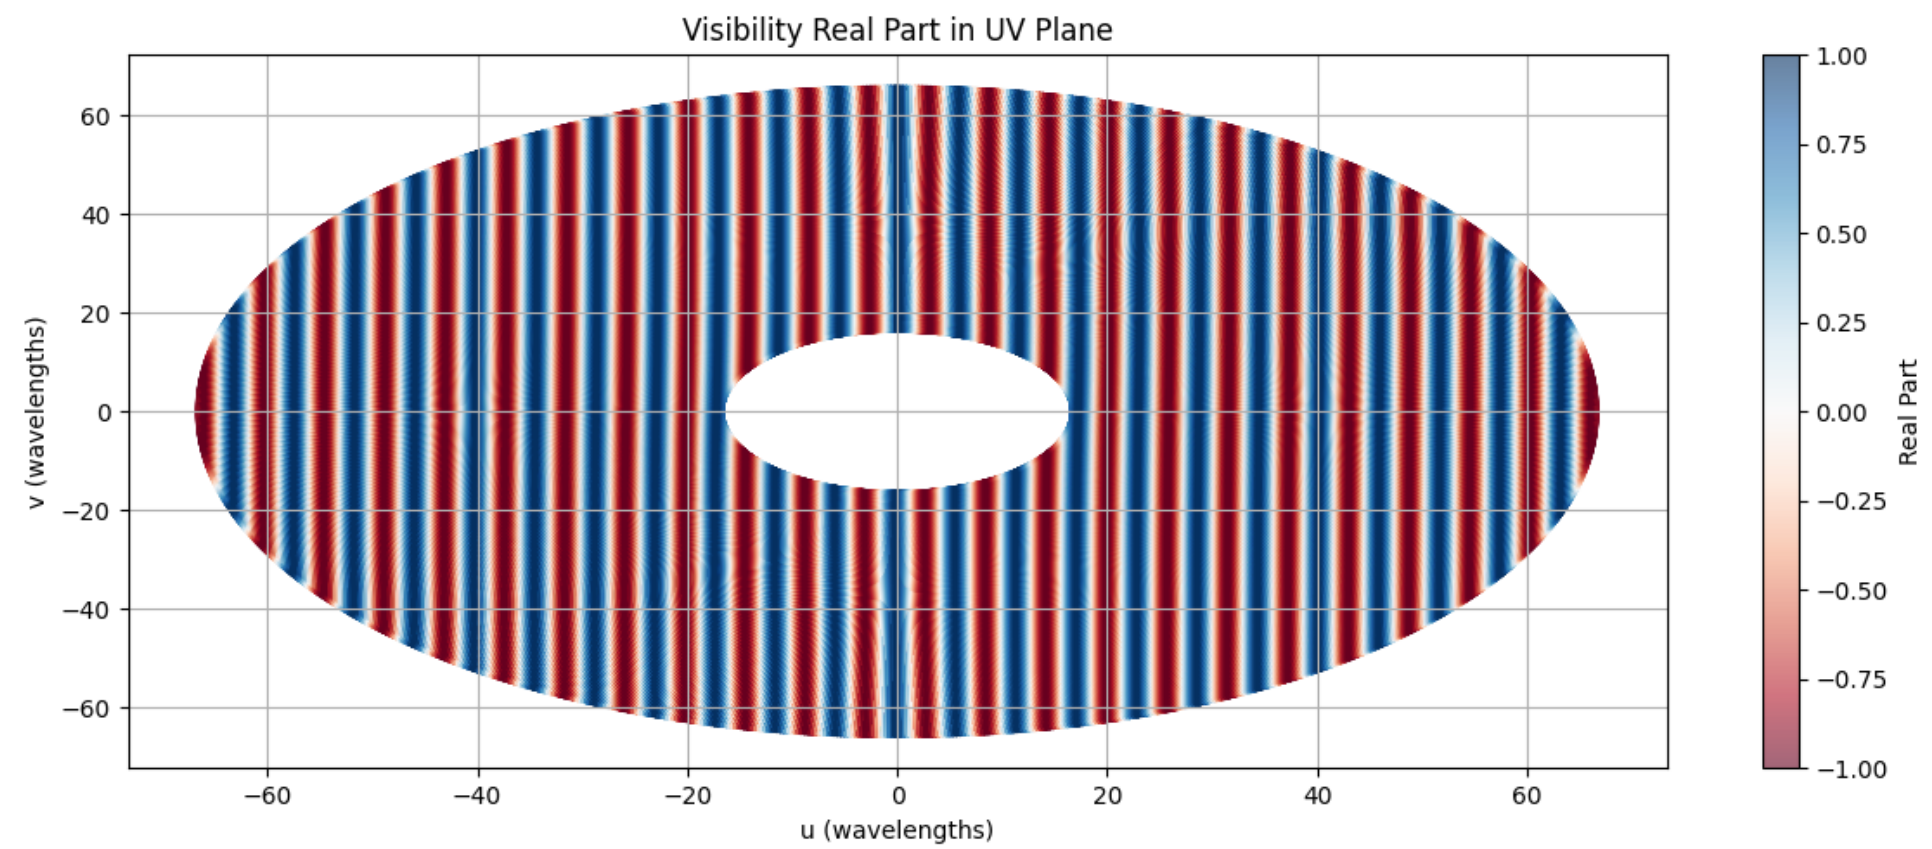
\includegraphics[width=1\textwidth]{task3/real.png}
    \label{fig:real}
    \end{figure}
\subsection{虚部uv图}
    \begin{figure}[htp]
    \centering
    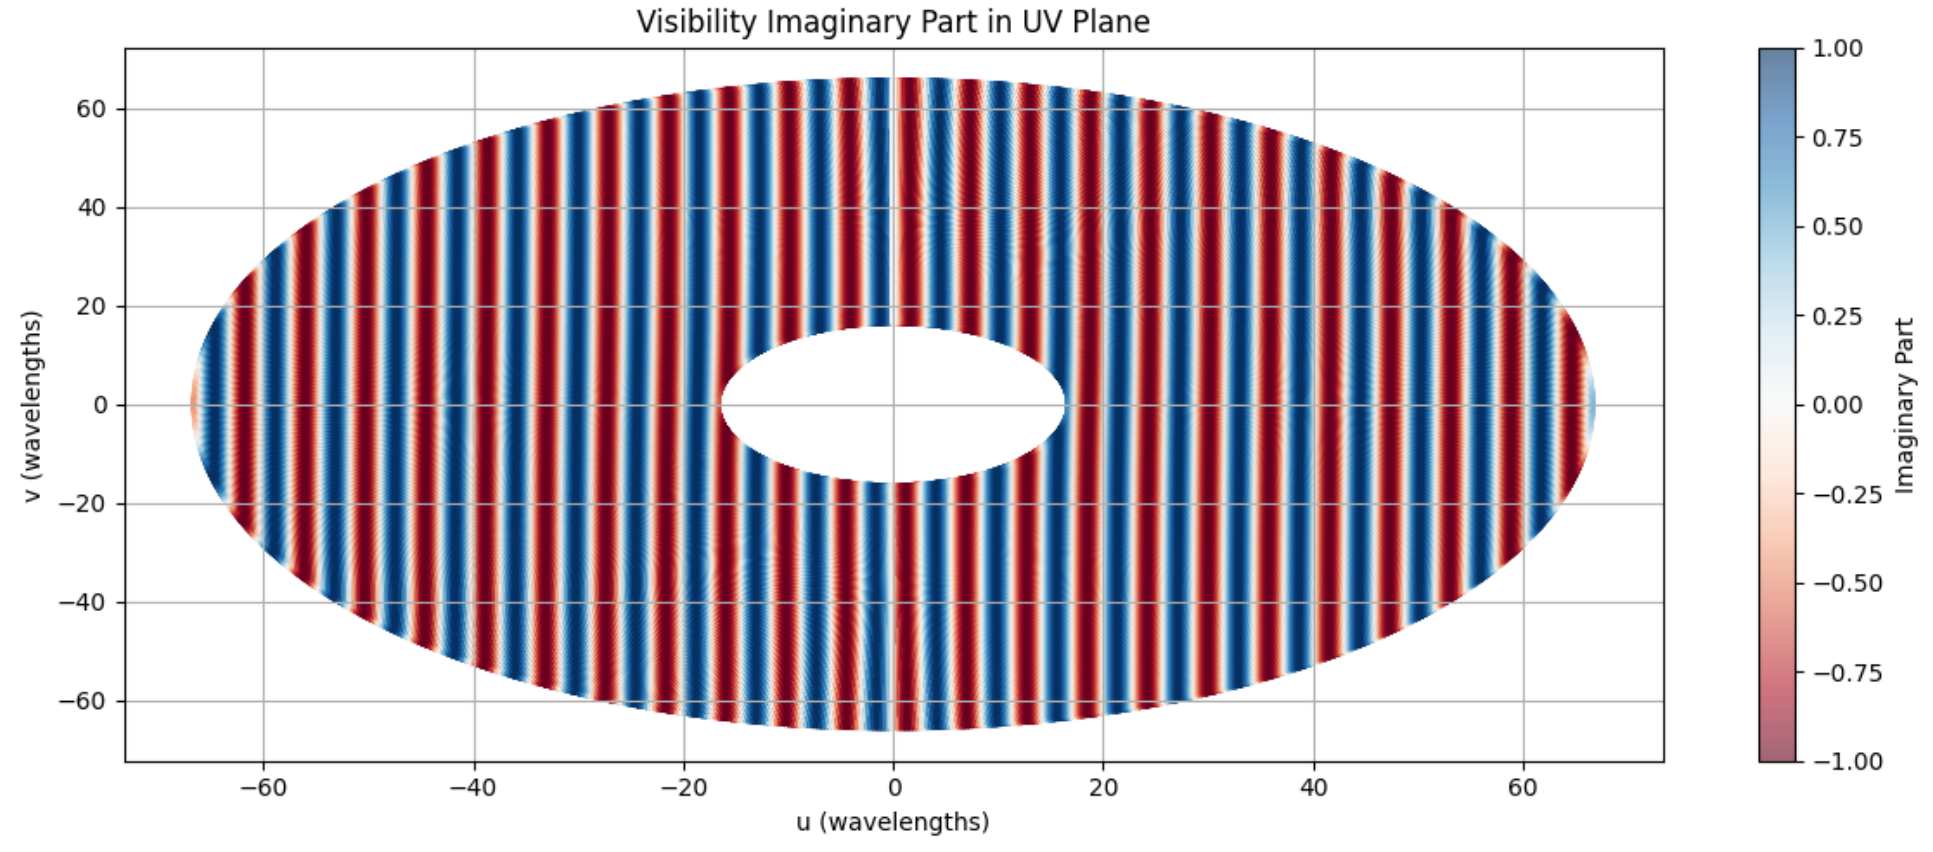
\includegraphics[width=1\textwidth]{task3/image.png}
    \label{fig:image}
    \end{figure}
\end{document}